\documentclass[german,11pt]{beamer}
% ------------------------------------------------------------------------------
% Packages
\usepackage[german,english,french]{babel}
\usepackage[T1]{fontenc}
\usepackage[utf8]{inputenc}
\usepackage{ragged2e}
\usepackage[normalem]{ulem}


\usepackage{listings}
\usepackage{color}
\usepackage{xcolor} 
\usepackage{plantuml}
% \usepackage{enumitem} \setitemize{leftmargin=*}   // Keine Aufzählung
\usepackage{pgfplots}

\usepackage{csquotes}

\pgfplotsset{compat=1.18}

\definecolor{dkgreen} {rgb}{0,0.6,0}
\definecolor{gray}{rgb}{0.5,0.5,0.5}
\definecolor{mauve}{rgb}{0.58,0,0.82}

\lstset{frame=tb,
  language=Java,
  aboveskip=3mm,
  belowskip=3mm,
  showstringspaces=false,
  columns=flexible,
  basicstyle={\small\ttfamily},
  numbers=none,
  numberstyle=\tiny\color{gray},
  keywordstyle=\color{blue},
  commentstyle=\color{dkgreen},
  stringstyle=\color{mauve},
  breaklines=true,
  breakatwhitespace=true,
  tabsize=3
}
% ------------------------------------------------------------------------------
% Parameters
\mode<presentation>{\usetheme{Luebeck}}
\setbeamertemplate{itemize items}[triangle]
\setbeamercovered{transparent}
\usecolortheme{dove}
\usefonttheme{serif}
\addtobeamertemplate{block begin}{}{\justifying}
% ToC
\AtBeginSection[] {
  \begin{frame}{Inhalt}
    \tableofcontents[currentsection]
  \end{frame}
}
% Headline
\makeatletter
\setbeamertemplate{headline}{%
  \leavevmode%
  \@tempdimb=2.4375ex%
  \ifnum\beamer@subsectionmax<\beamer@sectionmax%
    \multiply\@tempdimb by\beamer@sectionmax%
  \else%
    \multiply\@tempdimb by\beamer@subsectionmax%
  \fi%
  \ifdim\@tempdimb>0pt%
    \advance\@tempdimb by 1.825ex%
    \begin{beamercolorbox}[wd=.5\paperwidth,ht=\@tempdimb]{section in head/foot}%
      \vbox to\@tempdimb{\hfill\insertsectionnavigation{.3\paperwidth}\vfil}%
    \end{beamercolorbox}%
    \begin{beamercolorbox}[wd=.3\paperwidth,ht=\@tempdimb]{subsection in head/foot}%
      \vbox to\@tempdimb{\vfil\insertsubsectionnavigation{.5\paperwidth}\vfil}%
    \end{beamercolorbox}%
    \begin{beamercolorbox}[wd=.2\paperwidth,ht=\@tempdimb]{subsection in head/foot}%
      \vbox to\@tempdimb{\vfil\hfill
\includegraphics[height=1cm]{fig/graphics/logo.jpg}\vfil}
    \end{beamercolorbox}%    
  \fi%
}
\makeatother
% Footline
\makeatletter
\setbeamertemplate{footline}{%
  \leavevmode%
  \hbox{\begin{beamercolorbox}[wd=.5\paperwidth,ht=2.5ex,dp=1.125ex,leftskip=.3cm,rightskip=.3cm]{author in head/foot}%
    \usebeamerfont{author in head/foot}\insertshortdate \hfill \insertshortauthor
  \end{beamercolorbox}%
  \begin{beamercolorbox}[wd=.5\paperwidth,ht=2.5ex,dp=1.125ex,leftskip=.3cm,rightskip=.3cm plus1fil]{title in head/foot}%
    \usebeamerfont{title in head/foot}\insertshorttitle \hfill \insertframenumber\,/\,\inserttotalframenumber
  \end{beamercolorbox}}%
  \vskip0pt%
}
\makeatother

\addto\captionsenglish{% Replace "english" with the language you use
  \renewcommand{\contentsname}%
    {Whatever}%
}

% ------------------------------------------------------------------------------
% Infos
\title[VS]{Verteilte Systeme}
%\subtitle[Short subtitle]{Subtitle}
\author[BCK]{Prof. Dr. Martin Becke}
\date[0.9]{Version 0.9}
\institute[CaDS]{CaDS - HAW Hamburg}
%\logo{
\includegraphics[height=1cm]{fig/graphics/logo.jpg}}
% ------------------------------------------------------------------------------

% Document
\begin{document}

% ------------------------------------------------------------------------------
% Titlepage
\begin{frame}
  \titlepage{}
\end{frame}
% ------------------------------------------------------------------------------
% ToC
%\begin{frame}{Contents}
%  \tableofcontents
%\end{frame}
% ------------------------------------------------------------------------------
\section{Kommunikation}
%\section{Einleitung}
\subsection{Topologien}
\begin{frame}
  \frametitle{Topologien}
  \framesubtitle{Übersicht}
  \begin{itemize}
    \item One-to-All
    \item Tree-based (Spanning Tree)
    \item Flooding
    \item Gossip
  \end{itemize}
\end{frame}

\subsection{Protokolle}
\begin{frame}
  \frametitle{Protokolle}
  \framesubtitle{Produktive Protokolle - Beispiele}
  \begin{itemize}
    \item TCP/IP
    \item MQTT
    \item HTTP
  \end{itemize}
\end{frame}

\begin{frame}
  \frametitle{Protokolle}
  \framesubtitle{Basic Layers}
  \begin{itemize}
    \item Low-Level-Network-Programming
    \item High-Level-Network-Programming 
    \item Prompt Engineering (?)
  \end{itemize}
\end{frame}

\subsection{Allgemeine Diskussion}
\begin{frame}
  \frametitle{Kommunikation}
  \framesubtitle{Eigenschaften}
  \begin{itemize}
    \item Skalierbarkeit
    \item Fehlertoleranz
    \item Ausfallsicherheit
    \item Konsistenz
    \item Synchronisation
    \item Bandbreite, Latenz, Fehlerrate
    \item Kopplung
  \end{itemize}
\end{frame}

\begin{frame} [fragile]
  \frametitle{Auswahl nach Zerlegungsmethode}
  \framesubtitle{Ressourcen-orientierte}
  \begin{itemize}
    \item HTTP für die Ressourcen-orientierte Zerlegung
    \item de-facto die Basis für die Restful API
  \end{itemize}
  \begin{minipage}{\textwidth}
  \begin{lstlisting}[caption={Ressource anlegen (POST)},captionpos=b,label={lst:post}]
  POST /ressource HTTP/1.1
  Host: beispiel.com
  Content-Type: application/json
  Content-Length: 25
  {
    "name": "Beispielname"
  }
  \end{lstlisting}
  \end{minipage}
\end{frame}


\begin{frame} [fragile]
  \frametitle{Auswahl nach Zerlegungsmethode}
  \framesubtitle{Funktionale Zerlegung}
  \begin{itemize}
    \item Simple Object Access Protocol (SOAP) als Beispiel für 
  \end{itemize}
  \begin{minipage}{\textwidth}
  \begin{lstlisting}[caption={SOAP create},captionpos=b,label={lst:s_create}]
  <soapenv:Envelope xmlns:soapenv="http://schemas.xmlsoap.org/soap/envelope/" xmlns:per="http://example.com/person">
     <soapenv:Header/>
     <soapenv:Body>
        <per:CreatePersonRequest>
           <per:firstName>John</per:firstName>
           <per:lastName>Doe</per:lastName>
        </per:CreatePersonRequest>
     </soapenv:Body>
  </soapenv:Envelope>
  \end{lstlisting}
  \end{minipage}
\end{frame}

\subsection{REST}
\begin{frame}
  \frametitle{REST}
  \framesubtitle{Eigenschaften}
  \begin{itemize}
    \item Stateless
    \item Client-Server-Architektur
    \item Cachefähig
    \item Einheitliche Schnittstelle
    \item Ressourcenorientierung
  \end{itemize}
\end{frame}

\subsection{RESTful API}
\begin{frame}
  \frametitle{RESTful API}
  \framesubtitle{Eigenschaften angelehnt an REST}
  \begin{itemize}
    \item Einfachheit
    \item Zustandslos/ Skalierbar
    \item Interoperabilität (Client-Server-Architektur)
    \item Flexibilität
    \item Cachefähig
    \item Einheitliche Schnittstelle (HATEOAS)
    \item Ressourcenorientierung
  \end{itemize}
\end{frame}

\begin{frame}
  \frametitle{RESTful API}
  \framesubtitle{HATEOAS - Großes Missverständniss}
  \begin{itemize}
    \item Unklare Dokumentation
    \item Fehlende Standardisierung
    \item Begrenzter Einsatz
    \item Frontend-Technologien und Frameworks
  \end{itemize}
\end{frame}

\begin{frame} [fragile]
  \frametitle{RESTful API}
  \framesubtitle{HATEOAS - Beispiel}
  \begin{minipage}{\textwidth}
  \begin{lstlisting}[basicstyle=\tiny, caption={HATEOAS Lampe},captionpos=b,label={lst:hateoas}]
  {
    "id": 1,
    "status": "off",
    "_links": {
      "self": {
        "href": "https://api.example.com/lamps/1"
      },
      "turnOn": {
        "href": "https://api.example.com/lamps/1/actions/turnOn",
        "method": "PUT"
      },
      "setBrightness": {
        "href": "https://api.example.com/lamps/1/actions/setBrightness",
        "method": "PUT"
      },
      "setColor": {
        "href": "https://api.example.com/lamps/1/actions/setColor",
        "method": "PUT"
      }
    }
  }
  \end{lstlisting}
  \end{minipage}
\end{frame}


\begin{frame}
  \frametitle{RESTful API}
  \framesubtitle{Richardson Maturity Model}
  \begin{itemize}
    \item Level 0 - RPC over HTTP
    \item Level 1 - low level REST
    \item Level 2 - de-facto standard
    \item Level 3 - HATEOAS
  \end{itemize}
\end{frame}

\begin{frame}[fragile]
  \frametitle{Richardson Maturity Model}
  \framesubtitle{Level 0}
  Einzige URI: https://api.example.com/actions
  \\\\
  Aktionen werden durch unterschiedliche Parameter im Anfrage-Body bestimmt.
  \\\\
  \begin{minipage}{\textwidth}
  \begin{lstlisting}[caption={Level 0},captionpos=b,label={lst:level_0}]
  {
    "action": "getLamp",
    "lampId": 1
  }
  \end{lstlisting}
  \end{minipage}
\end{frame}

\begin{frame}[fragile]
  \frametitle{Richardson Maturity Model}
  \framesubtitle{Level 1}
  URI je Ressource: https://api.example.com/lamps/1
  \\\\
  Aber um die Lampe ein- oder auszuschalten, wird immer noch POST verwendet:
  \\\\
  \noindent\begin{minipage}{\textwidth}
  \begin{lstlisting}[caption={Level 1},captionpos=b,label={lst:level_1}]
  {
    "action": "turnOn"
  }
  \end{lstlisting}
  \end{minipage}
\end{frame}

\begin{frame}[fragile]
  \frametitle{Richardson Maturity Model}
  \framesubtitle{Level 2}
  URI je Ressource: https://api.example.com/lamps/1
  \\\\
  Verwendung von standardisierten HTTP-Methoden.
  \begin{itemize}
  \item Um Informationen über die Lampe abzurufen: GET https://api.example.com/lamps/1
  \item  Um die Lampe einzuschalten: PUT https://api.example.com/lamps/1/actions/turnOn
  \item Um die Lampe auszuschalten: PUT https://api.example.com/lamps/1/actions/turnOff
  \end{itemize}
\end{frame}

\subsection{Message Broker Protokolle}
\begin{frame}
  \frametitle{Message Broker Protokolle}
  \framesubtitle{IETF Kontext}
  \begin{itemize}
    \item AMQP
    \item STOMP
    \item MQTT
  \end{itemize}
\end{frame}

\begin{frame}
  \frametitle{Message Broker Protokolle}
  \framesubtitle{Beispiel MQTT}
  \begin{itemize}
    \item Leichtgewichtiges Publish-Subscribe-Protokoll
    \item Für eingeschränkte Umgebungen und Geräte mit begrenzter Rechenleistung
    \item Binäres Protokoll auf Basis von TCP/IP
    \item Gut geeignet ist für das Internet der Dinge (IoT)
    \item Geringe Latenz und geringer Bandbreitenverbrauch
    \item Geräte-zu-Geräte-Kommunikation
  \end{itemize}
\end{frame}

\begin{frame}
  \frametitle{Message Broker Protokoll}
  \framesubtitle{Message Broker}
  \begin{itemize}
    \item RabbitMQ 
    \item Beispiel eines Vergleichs \url{https://www.confluent.io/blog/kafka-fastest-messaging-system/}
    \item ZeroMQ (Broker-less)
    \item Beispiel MQTT Broker \url{https://github.com/hobbyquaker/awesome-mqtt}
    \item IBM MQ (Closed Source)
    \item HiveMQ (as a Service -Germany)
    \end{itemize}
\end{frame}

\begin{frame}
  \frametitle{Message Broker Protokolle}
  \framesubtitle{Beispiel Apache Kafka}
  \begin{itemize}
    \item Verteiltes Streaming-System
    \item Verarbeitung großer Datenmengen und Hochdurchsatz
    \item Skalierbares und fehlertolerantes System
    \item Verarbeitung und Speicherung von Datenströmen in Echtzeit
    \item Großen Datenmengen
    \item Kommunikation in groß angelegten, verteilten Anwendungen
  \end{itemize}
\end{frame}

\begin{frame}
  \frametitle{Message Broker Protokolle}
  \framesubtitle{Apache Kafka Alternativen}
  \begin{itemize}
    \item Apache Pulsar
    \item NATS Streaming 
    \item Amazon Kinesis
    \item Google Cloud Pub/Sub
    \item Redpanda
    \item Beispiel eines Vergleichs \url{https://www.confluent.io/blog/kafka-fastest-messaging-system/}
  \end{itemize}
\end{frame}

\begin{frame}
  \frametitle{Message Broker}
  \framesubtitle{Properitäre Alternative: IBM MQ}
  \begin{itemize}
    \item Message Queues
    \item Message Channel Agents
    \item Queue Manager
    \item Clients
  \end{itemize}
\end{frame}

\begin{frame}
  \frametitle{Message Broker}
  \framesubtitle{Priorizierung Nachrichten}
  \begin{itemize}
    \item Prioritätsniveaus
    \item Routing-Regeln
    \item Software-Tools
  \end{itemize}
\end{frame}

\begin{frame}
  \frametitle{Message Broker}
  \framesubtitle{Herausforderungen}
  \begin{itemize}
    \item Komplexität
    \item Ausfallsicherheit
    \item Skalierbarkeit
    \item Leistung
    \item Sicherheit
    \item Kompatibilität
    \item Wartung und Support
  \end{itemize}
\end{frame}

\subsection{RESTful API und States}
\begin{frame}
  \frametitle{RESTful API und States}
  \framesubtitle{Idee}
  \begin{itemize}
    \item REST ist ein resourcenorientiertes Designparadigma, das die Statemaschine in den Fokus stellt
    \item Fast ausschließlich jedes Programm besitzt eine Statemaschine
    \item States besitzen Eigenschaften und die Transitionen
    \item Es kann auch als Abstraktion bestehen
  \end{itemize}
\end{frame}

\begin{frame}
  \frametitle{RESTful API und States}
  \framesubtitle{Motivation}
  \begin{itemize}
    \item Konsistenz und Einfachheit
    \item Entkopplung von Client und Server
    \item Zustandslosigkeit
    \item Skalierbarkeit und Leistung
    \item Erweiterbarkeit und Anpassungsfähigkeit
    \item Einheitliche Schnittstelle
  \end{itemize}
\end{frame}

\begin{frame}[fragile]
  \frametitle{RESTful API und States}
  \framesubtitle{Fallbeispiel}

  \begin{figure}[!ht]
    \centering
    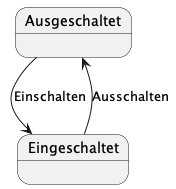
\includegraphics[width=0.35\textwidth]{fig/uml/lampe.png}
    \caption{Einfache FSM Lampe}
    \label{fig:lampe}
  \end{figure}
\end{frame}

\begin{frame}
  \frametitle{RESTful API und States}
  \framesubtitle{Fallbeispiel - Zustände abbilden}
    Ausgeschaltet: /lamp/off\\
    Eingeschaltet: /lamp/on\\
    \\\\
    HTTP-Verben für Zustandsübergänge:
    \\
    Einschalten: PUT /lamp/on\\
    Ausschalten: PUT /lamp/off
\end{frame}


\begin{frame}[fragile]
  \frametitle{RESTful API und States}
  \framesubtitle{Fallbeispiel - GET /lamp}
  \begin{minipage}{\textwidth}
  \begin{lstlisting}[caption={Fallbeispiel REST - an},captionpos=b,label={lst:rest_an}]
  {
    "state": "Eingeschaltet",
    "links": [
      {
        "rel": "self",
        "href": "/lamp/on",
        "method": "GET"
      },
      {
        "rel": "Ausschalten",
        "href": "/lamp/off",
        "method": "PUT"
      }
    ]
  }
  \end{lstlisting}
  \end{minipage}
\end{frame}

\begin{frame}[fragile]
  \frametitle{RESTful API und States}
  \framesubtitle{Fallbeispiel - LampModel}
  \begin{minipage}{\textwidth}
  \begin{lstlisting}[caption={LampModel},captionpos=b,label={lst:lamp_m}]
  class LampModel:
      def __init__(self):
          self.state = "AUS"

      def toggle(self):
          if self.state == "AUS":
              self.state = "EIN"
          else:
              self.state = "AUS"

      def get_state(self):
          return self.state

  \end{lstlisting}
  \end{minipage}
\end{frame}

\begin{frame}[fragile]
  \frametitle{RESTful API und States}
  \framesubtitle{Fallbeispiel - LampController}
    \begin{minipage}{\textwidth}
  \begin{lstlisting}[basicstyle=\tiny, caption={LampController},captionpos=b,label={lst:lamp_c}]
  class LampAdapter(Resource):
      def __init__(self, controller):
          self.controller = controller

      def get(self):
          response = {
              "state": self.controller.model.get_state(),
              "_links": {
                  "self": {"href": "/lamp"},
                  "on": {"href": "/lamp/on"},
                  "off": {"href": "/lamp/off"},
              }
          }
          return jsonify(response)

      def put(self):
          action = request.form.get("action")

          if action == "on":
              self.controller.on()
          elif action == "off":
              self.controller.off()

          response = {
              "state": self.controller.model.get_state(),
              "_links": {
                  "self": {"href": "/lamp"},
                  "on": {"href": "/lamp/on"},
                  "off": {"href": "/lamp/off"},
              }
          }
          return jsonify(response)
  \end{lstlisting}
  \end{minipage}
\end{frame}
\subsection{Allgemein}
\begin{frame}[fragile]
  \frametitle{RESTful API und States}
  \framesubtitle{Fallbeispiel - LampController}
  \begin{minipage}{\textwidth}
  \begin{lstlisting}[caption={Lamp REST APP},captionpos=b,label={lst:lamp_r}]
  from flask import Flask, jsonify, request
  from flask_restful import Resource, Api

  app = Flask(__name__)
  api = Api(app)

  lamp_model = LampModel()
  lamp_controller = LampController(lamp_model)
  lamp_adapter = LampAdapter(lamp_controller)

  api.add_resource(lamp_adapter, "/lamp", "/lamp/on", "/lamp/off")

  if __name__ == "__main__":
      app.run(debug=True)
  \end{lstlisting}
\end{minipage}
\end{frame}  



\begin{frame}
  \frametitle{RESTful API}
  \framesubtitle{Alternativen/Beispiele}
  \begin{itemize}
    \item CoAP
    \item XMPP
    \item DDS (Realtime Publish/Subscribe)
    \item OPC-UA (Industrielles Kommunikationsprotokoll)
    \item ROS
    \item Message Broker Protokolle
  \end{itemize}
\end{frame}



\begin{frame}
  \frametitle{Message Delivery}
  \framesubtitle{QoS}
  \begin{itemize}
    \item maybe (MQTT QoS 0)
    \item at-least-once (MQTT QoS 1)
    \item at-most-once
    \item exactly-once (MQTT QoS 2)
  \end{itemize}
\end{frame}

\begin{frame}
  \frametitle{Message Delivery}
  \framesubtitle{exactly-once}
  \begin{itemize}
    \item Zwei-Generäle-Problem (Gleich mehr)
    \item Unzuverlässige Kommunikation
    \item Unvorhersehbare Systemausfälle
    \item message processing vs  message delivery
  \end{itemize}
\end{frame}

\begin{frame}
  \frametitle{Byzantinische Generäle }
  \framesubtitle{Idee}
  \begin{itemize}
    \item Zwei-Generäle-Problem (Gruppenarbeit)
  \end{itemize}
\end{frame}


\begin{frame}
  \frametitle{Heartbeat}
  \framesubtitle{Idee}
  \begin{itemize}
    \item Ein periodisches Signal
    \item Verfügbarkeit und Erreichbarkeit
    \item Heartbeats in verteilten Systemen haben mehrere Funktionen
  \end{itemize}
\end{frame}

\begin{frame}
  \frametitle{Heartbeat}
  \framesubtitle{Ziel}
  \begin{itemize}
    \item Fehlererkennung
    \item Synchronisation
    \item Lastverteilung
  \end{itemize}
\end{frame}

\begin{frame}
  \frametitle{Heartbeat}
  \framesubtitle{Nachteile}
  \begin{itemize}
    \item Zusätzlichen Netzwerkverkehr
    \item False positives
    \item Skalierbarkeit
  \end{itemize}
\end{frame}

\begin{frame}
  \frametitle{Heartbeat}
  \framesubtitle{Konzepte}
  \begin{itemize}
    \item Zentral vs. de-zentral
    \item Hierarchisch vs flach
    \item In-Band- und Out-of-Band-Kommunikation
    \item Priorisierung von Heartbeat-Prozessen
    \item Adaptiven und lernenden Heartbeat-Systeme
  \end{itemize}
\end{frame}

\begin{frame}
  \frametitle{Multicast}
  \framesubtitle{Idee}
  \begin{itemize}
    \item Ansatz für effiziente und skalierbare Übertragung
    \item Schont Netzwerkressourcen
    \item Problem: Mapping auf physikalisches Netz
  \end{itemize}
\end{frame}

\begin{frame}
  \frametitle{Multicast}
  \framesubtitle{Ansätze}
  \begin{itemize}
    \item Application-Level Tree-Based Multicasting
    \item Datenbankreplikationen
    \item Redundanz
    \item Flooding-basiertes Multicasting
    \item Gossip-basiertes Multicasting
  \end{itemize}
\end{frame}

\begin{frame}
  \frametitle{Serialisierungsformate}
  \framesubtitle{Herausforderungen}
  \begin{itemize}
    \item Protocol Buffers
    \item MessagePack
    \item JSON
    \item XML
  \end{itemize}
\end{frame}

\begin{frame}
  \frametitle{Transport}
  \framesubtitle{Ideen}
  \begin{itemize}
    \item Push vs Pull
    \item Daten vs. Funktionen
  \end{itemize}
\end{frame}

\subsection{Namensräume}
\begin{frame}
  \frametitle{Namensräume}
  \framesubtitle{Begriffe}
  \begin{itemize}
    \item Name
    \item ID
    \item Adresse
  \end{itemize}
\end{frame}

\begin{frame}
  \frametitle{Service Discovery}
  \framesubtitle{Architektur I}
  \begin{itemize}
    \item Zentralen Architektur 
    \item Verteilte Service-Discovery-Architektur
    \item Hierarchische Service-Discovery-Architektur
  \end{itemize}
\end{frame}

\begin{frame}
  \frametitle{Service Discovery}
  \framesubtitle{Architektur II}
  \begin{itemize}
    \item Client-seitige Service-Discovery-Architektur
    \item Server-seitige Service-Discovery-Architektur
  \end{itemize}
\end{frame}

\begin{frame}
  \frametitle{Namensräume}
  \framesubtitle{Strukturen}
  \begin{itemize}
    \item Flacher Namensraum
    \item Hierarchischer Namensraum
    \item Attributbasierter Namensraum
  \end{itemize}
\end{frame}

\begin{frame}
  \frametitle{Naming}
  \framesubtitle{UUID}
  \begin{itemize}
    \item Version 1 (zeitbasiert)
    \begin{equation}
       = \text{Zeitstempel} + \text{Sequenznummer} + \text{MAC-Adresse}
    \end{equation}
    \item Version 2 (DCE Security)
         \begin{equation}
       = \text{Zeitstempel} + \text{Sequenznummer} + \text{MAC-Adresse} + text{DCE}
    \end{equation}
    \item Version 3 (MD5-Hash)
        \begin{equation}
        = \text{MD5-Hash}(\text{Namensraum-Identifikator} + \text{Name})
    \end{equation}
    \item Version 4 (zufällig)
    \item Version 5 (SHA-1-Hash)
  \end{itemize}
\end{frame}

\begin{frame}
  \frametitle{Locator/Identifier}
  \framesubtitle{Idee}
  \begin{itemize}
    \item Identifikator ist ein eindeutiges Label oder eine Kennung
    \item Lokator ist eine Information, für physischen Ort oder Adresse 
  \end{itemize}
\end{frame}

\begin{frame}
  \frametitle{Locator/Identifier}
  \framesubtitle{Protokolle}
  \begin{itemize}
    \item LISP
    \item HIP
    \item ILA
  \end{itemize}
  Anwendung:
  \begin{itemize}
    \item SIP
    \item Mobile IP
  \end{itemize}
\end{frame}


% ------------------------------------------------------------------------------
% Fin
\end{document}